% Options for packages loaded elsewhere
\PassOptionsToPackage{unicode}{hyperref}
\PassOptionsToPackage{hyphens}{url}
%
\documentclass[
]{article}
\usepackage{lmodern}
\usepackage{amssymb,amsmath}
\usepackage{ifxetex,ifluatex}
\ifnum 0\ifxetex 1\fi\ifluatex 1\fi=0 % if pdftex
  \usepackage[T1]{fontenc}
  \usepackage[utf8]{inputenc}
  \usepackage{textcomp} % provide euro and other symbols
\else % if luatex or xetex
  \usepackage{unicode-math}
  \defaultfontfeatures{Scale=MatchLowercase}
  \defaultfontfeatures[\rmfamily]{Ligatures=TeX,Scale=1}
\fi
% Use upquote if available, for straight quotes in verbatim environments
\IfFileExists{upquote.sty}{\usepackage{upquote}}{}
\IfFileExists{microtype.sty}{% use microtype if available
  \usepackage[]{microtype}
  \UseMicrotypeSet[protrusion]{basicmath} % disable protrusion for tt fonts
}{}
\makeatletter
\@ifundefined{KOMAClassName}{% if non-KOMA class
  \IfFileExists{parskip.sty}{%
    \usepackage{parskip}
  }{% else
    \setlength{\parindent}{0pt}
    \setlength{\parskip}{6pt plus 2pt minus 1pt}}
}{% if KOMA class
  \KOMAoptions{parskip=half}}
\makeatother
\usepackage{xcolor}
\IfFileExists{xurl.sty}{\usepackage{xurl}}{} % add URL line breaks if available
\IfFileExists{bookmark.sty}{\usepackage{bookmark}}{\usepackage{hyperref}}
\hypersetup{
  pdftitle={Forecasting hospitalizations due to COVID-19 in South Dakota},
  hidelinks,
  pdfcreator={LaTeX via pandoc}}
\urlstyle{same} % disable monospaced font for URLs
\usepackage[margin=1in]{geometry}
\usepackage{longtable,booktabs}
% Correct order of tables after \paragraph or \subparagraph
\usepackage{etoolbox}
\makeatletter
\patchcmd\longtable{\par}{\if@noskipsec\mbox{}\fi\par}{}{}
\makeatother
% Allow footnotes in longtable head/foot
\IfFileExists{footnotehyper.sty}{\usepackage{footnotehyper}}{\usepackage{footnote}}
\makesavenoteenv{longtable}
\usepackage{graphicx,grffile}
\makeatletter
\def\maxwidth{\ifdim\Gin@nat@width>\linewidth\linewidth\else\Gin@nat@width\fi}
\def\maxheight{\ifdim\Gin@nat@height>\textheight\textheight\else\Gin@nat@height\fi}
\makeatother
% Scale images if necessary, so that they will not overflow the page
% margins by default, and it is still possible to overwrite the defaults
% using explicit options in \includegraphics[width, height, ...]{}
\setkeys{Gin}{width=\maxwidth,height=\maxheight,keepaspectratio}
% Set default figure placement to htbp
\makeatletter
\def\fps@figure{htbp}
\makeatother
\setlength{\emergencystretch}{3em} % prevent overfull lines
\providecommand{\tightlist}{%
  \setlength{\itemsep}{0pt}\setlength{\parskip}{0pt}}
\setcounter{secnumdepth}{5}
\usepackage{booktabs}
\usepackage{longtable}
\usepackage{array}
\usepackage{multirow}
\usepackage{wrapfig}
\usepackage{float}
\usepackage{colortbl}
\usepackage{pdflscape}
\usepackage{tabu}
\usepackage{threeparttable}
\usepackage{threeparttablex}
\usepackage[normalem]{ulem}
\usepackage{makecell}
\usepackage{xcolor}

\title{Forecasting hospitalizations due to COVID-19 in South Dakota}
\author{}
\date{\vspace{-2.5em}}

\begin{document}
\maketitle

\hypertarget{authors}{%
\section{Authors}\label{authors}}

\emph{Jeff Wesner}\textsuperscript{1}, \emph{Dan Van Peursem}\textsuperscript{2}, \emph{Jose Flores}\textsuperscript{2,3}, \emph{Yuhlong Lio}\textsuperscript{2}, \emph{Chelsea Wesner}\^{}3

University of South Dakota

\textsuperscript{1}Department of Biology, \textsuperscript{2}Department of Mathematical Sciences, \textsuperscript{3}Department of Computer Science, \^{}3Master of Public Health Program

\href{mailto:Jeff.Wesner@usd.edu}{\nolinkurl{Jeff.Wesner@usd.edu}}

\hypertarget{abstract}{%
\section{Abstract}\label{abstract}}

Anticipating the number of hospital beds needed for patients with COVID-19 remains a challenge. Early efforts to predict hospital bed needs focused on deriving predictions from SIR models, largely at the level of countries, provinces, or states. In the United States, these models rely on data reported by state health agencies. However, predictive disease and hospitalization dynamics at the state level is complicated by geographic variation in disease parameters. In addition it is difficult to make forecasts early in a pandemic due to minimal data. However, Bayesian approaches that allow models to be specified with informed prior information from areas that have already completed a disease curve can serve as prior estimates for areas that are beginning their curve. Here, we used a Bayesian non-linear regression (Weibull function) to forecast cumulative and active COVID-19 hospitalizations for South Dakota, USA. As expected, early forecasts were dominated by prior information, which we derived from New York City. Importantly, hospitalization trends also differed within South Dakota due to early peaks in urban Minnehaha County, followed by later peaks in other rural areas of the state. Combining these trends in an interaction model led to altered forecasts with relevant policy implications.

\hypertarget{introduction}{%
\section{Introduction}\label{introduction}}

The novel coronavirus (SARS-CoV-2) was first detected in December 2019 in Wuhan, China and has since spread globally. The disease caused by SARS-CoV-2 (COVID-19) can lead to hospitalization or death in all age groups, but particularly in older age groups with comorbidities such as hypertension, obesity, and diabetes (Richardson et al. 2020). For example,in France Salje et al. (2020) estimated that 3.6\% of infected people become hospitalized, but that rate varies from a low of 0.001\% to 10.1\% for individuals that are \textless20 years old versus those \textgreater80 years old, respectively. A central challenge for hospitals is predicting how many hospitalizations will occur due to COVID-19, and whether hospital capacities will be exceeded.
Predicting hospitalization needs due to COVID-19 may be particularly challenging in rural areas. For example, relative to urban areas, rural communities in the U.S. have reduced access to health care (Research and Quality 2016) and increased mortality from chronic diseases (Moy et al. 2017), both of which are key risk factors for COVID-19. South Dakota is among the most rural states in the U.S. with a 2017 population estimate of 869,666 (Bureau 2017). Of South Dakota's 66 counties, 52\% are frontier (with \textless15.5 persons per square kilometer) and 32\% encompass or are comprised of reservation lands representing nine federally recognized tribes. Communiites in rural areas also tend to have an older poplution. For example, among 56 U.S. counties with the largest proportion of people ages \textgreater85, all but 2 counties are rural and a county in South Dakota ranks first (Henning-Smith et al. 2020). South Dakota's public health infrastructure is limited with a centralized state department of health and a single public nurse in each county to support the delivery of public health interventions and resources. Nearly 80\% of nonprofit hospitals in South Dakota are critical access hospitals with 25 or fewer acute inpatient beds (``DOH Provider List'' n.d.), and acess to medical facilities with an intensive care unit (ICU) and ventilators is limited in rural areas (Casey et al. 2018).
To our knowledge, there are no published studies that model hospitalizations due to COVID-19 in rural and low resource settings. Developing new ways to model infectious disease outbreaks in jurisdictions with limited public health and health care infrastructure is critical to preventing and reducing mortality and morbidity in communities that are at high risk COVID-19. Here, we modeled cumulative hospitalizations in and urban and rural populations within South Dakota using a Bayesian non-linear Weibull function. Because early predictions in a disease outbreak are critical for planning, but also are data limited, we used informed priors from New York City, which began its hospitalization curve before South Dakota. While New York City is not a rural area, the use of informed prior distributions allowed our model to make reasonable, though highly uncertain, forecasts of hospitalizations in a rural setting.

\hypertarget{methods}{%
\section{Methods}\label{methods}}

\textbf{Data Retrieval}

We obtained data on cumulative hospitalizations and active hospitalizations (number hospitalized on a given day) from the data dashboard for the South Dakota Department of Health (SD DOH) - \url{https://doh.sd.gov/news/Coronavirus.aspx\#SD}. Data for cumulative hospitalizations began on 2020-03-08 and were entered by hand into a .csv each day (SD DOH only reports totals for the current day, not a timeline). Data for active hospitalizations were not released until 2020-04-20, when 56 people were actively hospitalized. Beginning on that date, we also updated our .csv with active hospitalizations each day.
When data collection began, most cases and hospitalizations were located in a single county in South Dakota, Minnehaha County. Therefore, during data collection, we noted hospitalizations in Minnehaha County versus the rest of South Dakota to capture any potential divergent trends. For these two groups, data are only available for cumulative hospitalizations, not for active hospitalizations.

\textbf{Models}

We estimated the cumulative hospitalizations using a Bayesian non-linear sigmoid model in which hospitalizations were modeled as a function of time using the Weibull function (Yang, Kozak, and Smith 1978; Narushin and Takma 2003). The Weibull function is derived from the Weibull cumulative distribution (Weibull (1951)) and has been used widely in biology to model growth curves {[}pielou\_usefulness\_1981{]}. We chose the Weibull function because it is more flexible than the logistic function and is asymmetric around the inflection point (Yang, Kozak, and Smith 1978; Kumar, n.d.). We fit the Weibull function to two sets of data that describe 1) the cumulative hospitalizations for the state of South Dakota and 2) the cumulative hospitalizations for subgroups of Minnehaha County and the rest of South Dakota. Becuase the data were counts with positive outcomes, we used a Poisson likelihood with a log-link.

\emph{Model 1}

\[y_i \sim Poisson(\lambda_i)\]
\[log\lambda_i = \alpha_i(1 - exp(-\frac{x_i}{\beta_i})^{\gamma_i})\]

\[\alpha \sim Gamma(64,8)\]
\[\beta \sim Gamma(2.9, 0.18)\]
\[\gamma \sim Gamma(5.8,4.8)\]

where \emph{y\_i} is the cumulative number of people hospitalized in South Dakota on the \emph{ith} date, \(\alpha\) is the asymptote, \(\beta\) is the inflection point, and \(\gamma\) is the slope at the inflection point. Gamma priors were used because each parameter must be positive and continuous.
Informative prior distributions were derived from the cumulative hospitalization curve in New York City (NYC Department of Health, \url{https://www1.nyc.gov/site/doh/covid/covid-19-data.page}). We derived the priors from New York City because NYC had nearly completed its hospitalization curve when South Dakota's was still beginning and because the data were available as a timeline (many states either have not reported temporal hospitalization data or have not made the data easily extractable).
To derive prior distributions for South Dakota, we first fit the aforementioned model to NYC's hospitalization curve. Before fitting the model, we multiplied NYC hospitalizations by 0.10 to put them on the scale of South Dakota's population (which is \textasciitilde10\% of NYC's population). We then fit the model to these adjusted hospitalizations using prior values of \emph{Gamma}(1.2, 0.1) for \(\alpha\), \emph{Gamma}(0.25, 0.005) for \(\beta\), and \emph{Gamma}(1.4, 0.3) for \(\gamma\). Those reflect prior distributions with wide standard deviations that would represent a potential overload of South Dakota's \textasciitilde{} 2000 hospital beds: 10,000 +/- 5000 (mean +/- sd) for \(\alpha\), 50 +/- 100 for \(\beta\), and 100 +/- 50 for \(\gamma\).

\emph{Model 2}

Within South Dakota, Minnehaha County is the most densely populated area of the state, containing the largest city in South Dakota - Sioux Falls, SD. Daily tracking revealed a clear separation between trends (in both cases and hospitalizations) in Minnehaha County compared to trends outside of Minnehaha County. To capture these trends, we fit the same model as before, but included an interaction with two levels (Minnehaha County or Outside Minnehaha County) for each of the three parameters.

\[y_i \sim Poisson(\lambda_i)\]
\[log\lambda_i = \alpha_j(1 - exp(-\frac{x_i}{\beta_j})^{\gamma_j})\]
\[\alpha_j = \alpha_{minn} + \alpha_{rest}r_i\]
\[\beta_j = \beta_{minn} + \beta_{rest}r_i\]
\[\gamma_j = \gamma_{minn} + \gamma_{rest}r_i\]
\[\alpha_{minn} \sim Gamma(49,7)\]
\[\alpha_{rest} \sim Normal(0,1)\]
\[\beta_{minn} \sim Gamma(2.9, 0.18)\]
\[\beta_{rest} \sim Normal(0, 5)\]
\[\gamma_{minn} \sim Gamma(5.8, 4.8)\]
\[\gamma_{rest} \sim Normal(0,0.5)\]

where \emph{y\_i} is the cumulative number of people hospitalized in each \emph{i} date (\emph{x\_i}), \(\alpha_j, \beta_j,\) and \(\gamma_j\) are the parameters for each \emph{j} group (Minnehaha County or the Rest of South Dakota), \(X_{minn}\) are the priors for each X parameter (\(\alpha\), \(\beta\), \(\gamma\)), \(X_{rest}\) are the priors for the difference in parameter values between Minnehaha and the Rest of South Dakota, and \(r_i\) is an indicator variable that is 0 if the data are in Minnehaha County and 1 otherwise.
As before, prior values were chosen from a combination of prior information from NYC and from prior predictive simulation (Gabry et al. 2019). To do this, we simulated 300 cumulative hospitalization curves with mean values for each parameter derived from the fit of the NYC model. Because NYC has both a higher absolute population size and a higher population density (by 10-fold) than South Dakota, we adjusted prior means and standard deviations so that the prior predictive distributions estimated hospitalizations to have a maximum that is slighly below the maximum of NYC, but with standard deviations that still include positive prior probability for some extreme prediction (e.g., 50,000 cumulative hospitalizations). Figure \ref{prior_plots:plot} shows the prior predictions for both models.

\emph{Hamiltonian Monte Carlo}

Each model aforementioned was specified in R (version 3.6.3; R Core Team 2020) using the \emph{brms} package (Burkner, n.d.). Posterior sampling was performed using Hamiltonian Monte Carlo in \emph{rstan} (version 2.19.2, (Carpenter et al. 2017)). We fit four chains, each with 2000 iterations, discarding the first 1000 iterations of each chain as warm-up. Warm-up samples are similar to burn-in sampling, but are used in this case as an optimizer for the HMC algorithm. Chains were checked for convergence using trace plots to assure overlap (\emph{Supplementary Information}), and by ensuring that the Gelman-Rubin convergence diagnostic (\emph{r-hat}) was \textless{} 1.1 (Gelman and Rubin 1992).

\emph{Parameter change over time}

To determine how parameter values changed over time as data are added, we fit the model every twenty days and plotted the posterior distributions of parameter values against time.

\emph{Posterior prediction}
To forecast cumulative hospitalizations, we used the posterior predictive distributions from each model by first solving for the fitted values across each iteration of the posterior:

\[yfit_i^{(k)} = exp(\alpha_i^{(k)}(1 - exp(-\frac{x_i}{\beta_i^{(k)}})^{\gamma_i^{(k)}}))\]
where \emph{k} is the \(k^{th}\) iteration from the posterior distribution and \emph{i} is the \(i^{th}\) date. Posterior predicted values were estimated by drawing each \(ypred_i^{(k)}\) from the Poisson distribution:

\[ypred_i^{(k)} = Poisson(yfit_i^{(k)})\]
We then summarized the mean, median, standard deviation and credible intervals (50 and 95\%) across the posterior distribution of fitted and predicted values. For visualization, we plotted fitted values within the range of the data and predicted values beyond the range of the data.

\emph{Estimating Active Hospitalizations}

To estimate active hospitalizations from the cumulative hospitalization curve, we first derived daily incidence \(\phi\) for each iteration of \(yfit_{ki}\) in which

\[\phi_{ki} = yfit_i^{(k)} - yfit_{i-1}^{(k)}\]

We then summed incidence over the previous 5, 10, 12, or 15 days to estimate variable lengths of hospital stays:
\[\omega_i^{(k)} = \phi_i^{(k)} + \phi_{i-1}^{(k)} + \phi_{i-2}^{(k)}...\phi_{i-n}^{(k)}\]

where \(\omega_i^{(k)}\) is the number of people actively hospitalized on the \(i^th\) day for the \(k^th\) iteration, \(\phi_i^{(k)}\) is the incidence on the \(i^th\) day for the \(k^th\) iteration and \emph{n} is 5, 10, 12, or 15 (NEED CITATION).

We then plotted these predictions against active hospitalizations reported by the South Dakota Department of Health. For the group levels (\emph{Model 2}), we performed the same calculations as above, but for each group. In addition, we also estimated the state-level hospitalizations from \emph{Model 2} by summing the predictions from each group. This allowed us to compare predictions when only state-level data were available versus predictions with data available for different areas of the state.

\hypertarget{results}{%
\section{Results}\label{results}}

At the state level, model 1 predicted a total of 762 hospitalizations (median) in South Dakota (90\% CrI: 715 - 816, Table 2). The inflection point was predicted at 28 days after the first hospitalization, suggesting that the peak rate of hospitalizations occurred around April 11, 2020. In contrast, the model with group-level effects separating trends in Minnehaha County clearly showed that hospitalizations trends differed in Minnehaha County verses the rest of South Dakota (Figure \ref{post_all_plot:plot}). In Minnehaha County, the inflection point occurred around day 23 and revealed an asymptote of 316 hospitalizations (90\% CrI: 307-324). In the rest of South Dakota, the inflection point occurred \textasciitilde40 days later (day 62, Figure \ref{post_all_plot:plot}). Similarly, the maximum cumulative hospitalizations in the rest of South Dakota are estimated at a median of \textasciitilde785, but with large uncertainty (90\% CrI: 673-929, Table 2).

As expected the uncertainty in parameter values improved over time as data were added to the model. The largest improvement appeared to occur during the model run on day 60, when all parameter values appeared to stabilize (Figure \ref{param_time_plot:plot}).

Converting the cumulative curve to estimate the number of people actively hospitalized yields a maximum estimate of \textasciitilde100 people actively hospitalized. This estimate is derived from the assumption that an average patient will spend 10 days in the hospital. That assumption appeared to best approximate the state reported data best (Figure \ref{active_daily_group:plot}). However, the state reported data also appear to be staying consistent at around 90 people hospitalized even when model 1 predicts that active hospitalizations should be declining (Figure \ref{active_daily_group:plot}). It is possible that some of the difference is due to underlying differences in hospitalizations in the two subgroups, but active hospitalization data are only available for the state, so we are unable to assess the accuracy of the group-level predictions (Figure \ref{active_daily_group:plot}).

\hypertarget{discussion}{%
\section{Discussion}\label{discussion}}

The most important result of this study is that modeling trends separately in urban versus rural parts of a state population reveal different projections of cumulative hospitalizations than if modeled only using state-level data. In particular, the model with urban vs.~rural groups predicts that Minnehaha County will attain a maximum of \textasciitilde316 hospitalizations, while areas outside of Minnehaha will attain a maximum of \textasciitilde785. That results in approximately \textasciitilde1000 people cumulatively hospitalized. In contrast, the model with only state-level data indicates a 24\% smaller number of total people hospitalized (762).

In addition to differences in maximum hospitalizations, the models predict different trends of active hospitalizations. Active hospitalizations are more relevant than cumulative hospitalizations for measuring hospital capacity. They have been modeled for the COVID pandemic in a variety of ways with many states adopting a version of an SIR model, such as the CHIME model (E. Weissman et al. 2020). One challenge with estimating hospitalizations using an SIR-based approach is that they require estimates of a number of transition probabilities to convert infections into hospitalizations. These include estimating the proportion of infected people that become symptomatic, the proportion of those that require hospitalization, the proportion of those that seek hospitalization, the time lag between viral infection as modeled in an SIR, symptom onset, and actual hospitalization (E. Weissman et al. 2020; Imperial College COVID-19 Response Team et al. 2020). Early in an epidemic, when hospitalization data are scarce or absent, these models are essential for predicting possible hospitalization scenarios. However, once enough data are available on hospitalizations, it is possible to model the hospitalization curve directly, as we have done here.

Though we did not attempt to predict COVID-19 infections in South Dakota, it may be possible to use our approach to do so by treating infections as a latent variable that leads to subsequent hospitalizations. Imperial College COVID-19 Response Team et al. (2020) provide an exmaple of this approach using COVID-19-related deaths rather than hospitalizations. By modeling the dynamics of deaths, they estimated a time-varying reproduction number (\(R_t\)), which was used to estimate the number of positive cases. Using deaths (or hospitalizations) to estimate infection dynamics may help to overcome limitations in testing capacity, which in turn lead to difficulty in linking publically-reported testing results to true population-level infection rates. This is particularly true in the United States, which has limited testing capacity and no centrally coordinated testing program (Schneider 2020).

An advantage to the Bayesian approach is that we can use prior values of parameters in a model to fit a model with limited data. In our case, those parameters were conveniently available from New York City. However, if we were modeling a hospitalizaton curve that had no prior estimates, then we might derive priors from another epidemic that had similar disease symptoms(NOT THE RIGHT WORD..) or use prior predictive simulation to bound the model to reasonable prior predictions. The second method is the approach outlined in Gabry et al. (2019), who demonstrated the importance visualization in choosing prior parameters. In particular, becuase the prior distributions for individual parameters may not be known or are difficult to interpret without consideration of the likelihood (Gelman, Simpson, and Betancourt 2017), it is important to assess the the implications of prior choices using the prior predictive distribution (i.e.~simulating potential from the prior distrbutions alone) (Gabry et al. 2019) (Figure 1). In our model, data simulated from the prior helped to confirm that our model was specified in a way that included a wide range of hospitalization trajectories (Figure 1), but excluded extreme values that might have come from more diffuse priors, such as projecting asymptotes with hospitalizations that are higher than the population of South Dakota.

\hypertarget{acknowledgments}{%
\section{Acknowledgments}\label{acknowledgments}}

We declare no conflicts of interest. We thank the South Dakota Department of Health for making the hospitalization data publically available. This work is not affiliated with any funding agency.

\hypertarget{references}{%
\section{References}\label{references}}

\hypertarget{refs}{}
\leavevmode\hypertarget{ref-bureau_acs_2017}{}%
Bureau, US Census. 2017. ``ACS Demographic and Housing Estimates, 2013--2017 American Community Survey 5-Year Estimates.''

\leavevmode\hypertarget{ref-burkner_brms_nodate}{}%
Burkner, Paul-Christian. n.d. ``Brms: An R Package for Bayesian Generalized Linear Mixed Models Using Stan,'' 22.

\leavevmode\hypertarget{ref-carpenter_stan_2017}{}%
Carpenter, Bob, Andrew Gelman, Matthew D. Hoffman, Daniel Lee, Ben Goodrich, Michael Betancourt, Marcus Brubaker, Jiqiang Guo, Peter Li, and Allen Riddell. 2017. ``\emph{Stan} : A Probabilistic Programming Language.'' \emph{Journal of Statistical Software} 76 (1). \url{https://doi.org/10.18637/jss.v076.i01}.

\leavevmode\hypertarget{ref-casey_availability_2018}{}%
Casey, Michelle, Alex Evenson, Ira Moscovice, and Zhengtian Wu. 2018. ``Availability of Respiratory Care Services in Critical Access and Rural Hospitals.'' \emph{Policy Brief.(June 2018). University of Minnesota Rural Health Research Center. Retrieved from Http://Rhrc. Umn. Edu/Wpcontent/Files\_mf/1530149057UMNpolicybriefAvailabilityofRespiratoryCareServices. Pdf}.

\leavevmode\hypertarget{ref-noauthor_doh_nodate}{}%
``DOH Provider List.'' n.d. Accessed July 6, 2020. \url{https://apps.sd.gov/ph04lassnet/rptPH04LicenseList.Aspx}.

\leavevmode\hypertarget{ref-e_weissman_locally_2020}{}%
E. Weissman, Gary, Andrew Crane-Droesch, Corey Chivers, ThaiBinh Luong, Asaf Hanish, Michael Z. Levy, Jason Lubken, et al. 2020. ``Locally Informed Simulation to Predict Hospital Capacity Needs During the COVID-19 Pandemic.'' \emph{Annals of Internal Medicine}, April. \url{https://doi.org/10.7326/M20-1260}.

\leavevmode\hypertarget{ref-gabry_visualization_2019}{}%
Gabry, Jonah, Daniel Simpson, Aki Vehtari, Michael Betancourt, and Andrew Gelman. 2019. ``Visualization in Bayesian Workflow.'' \emph{Journal of the Royal Statistical Society: Series A (Statistics in Society)} 182 (2): 389--402. \url{https://doi.org/10.1111/rssa.12378}.

\leavevmode\hypertarget{ref-gelman_inference_1992}{}%
Gelman, Andrew, and Donald B. Rubin. 1992. ``Inference from Iterative Simulation Using Multiple Sequences.'' \emph{Statistical Science} 7 (4): 457--72. \url{https://doi.org/10.1214/ss/1177011136}.

\leavevmode\hypertarget{ref-gelman_prior_2017}{}%
Gelman, Andrew, Daniel Simpson, and Michael Betancourt. 2017. ``The Prior Can Often Only Be Understood in the Context of the Likelihood.'' \emph{Entropy} 19 (10): 555. \url{https://doi.org/10.3390/e19100555}.

\leavevmode\hypertarget{ref-henning-smith_characteristics_2020}{}%
Henning-Smith, Carrie, Megan Lahr, Jonathan Schroeder, Cody Tuttle, and Samantha Mills. 2020. ``Characteristics of Counties with the Highest Proportion of the Oldest Old.''

\leavevmode\hypertarget{ref-imperial_college_covid-19_response_team_estimating_2020}{}%
Imperial College COVID-19 Response Team, Seth Flaxman, Swapnil Mishra, Axel Gandy, H. Juliette T. Unwin, Thomas A. Mellan, Helen Coupland, et al. 2020. ``Estimating the Effects of Non-Pharmaceutical Interventions on COVID-19 in Europe.'' \emph{Nature}, June. \url{https://doi.org/10.1038/s41586-020-2405-7}.

\leavevmode\hypertarget{ref-kumar_epidemiological_nodate}{}%
Kumar, Jagadish. n.d. ``Epidemiological Study of Novel Coronavirus (COVID-19),'' 9.

\leavevmode\hypertarget{ref-moy_leading_2017}{}%
Moy, Ernest, Macarena C Garcia, Brigham Bastian, Lauren M Rossen, Deborah D Ingram, Mark Faul, Greta M Massetti, et al. 2017. ``Leading Causes of Death in Nonmetropolitan and Metropolitan Areas---United States, 1999--2014.'' \emph{MMWR Surveillance Summaries} 66 (1): 1.

\leavevmode\hypertarget{ref-narushin_sigmoid_2003}{}%
Narushin, V. G, and C Takma. 2003. ``Sigmoid Model for the Evaluation of Growth and Production Curves in Laying Hens.'' \emph{Biosystems Engineering} 84 (3): 343--48. \url{https://doi.org/10.1016/S1537-5110(02)00286-6}.

\leavevmode\hypertarget{ref-research_national_2016}{}%
Research, Agency for Healthcare, and Quality. 2016. ``National Healthcare Quality and Disparities Report Chartbook on Access to Health Care.''

\leavevmode\hypertarget{ref-richardson_presenting_2020}{}%
Richardson, Safiya, Jamie S. Hirsch, Mangala Narasimhan, James M. Crawford, Thomas McGinn, Karina W. Davidson, and the Northwell COVID-19 Research Consortium, et al. 2020. ``Presenting Characteristics, Comorbidities, and Outcomes Among 5700 Patients Hospitalized with COVID-19 in the New York City Area.'' \emph{JAMA} 323 (20): 2052. \url{https://doi.org/10.1001/jama.2020.6775}.

\leavevmode\hypertarget{ref-salje_estimating_2020}{}%
Salje, Henrik, Cécile Tran Kiem, Noémie Lefrancq, Noémie Courtejoie, Paolo Bosetti, Juliette Paireau, Alessio Andronico, et al. 2020. ``Estimating the Burden of SARS-CoV-2 in France.'' \emph{Science}, May, eabc3517. \url{https://doi.org/10.1126/science.abc3517}.

\leavevmode\hypertarget{ref-schneider_failing_2020}{}%
Schneider, Eric C. 2020. ``Failing the Test --- the Tragic Data Gap Undermining the U.S. Pandemic Response.'' \emph{New England Journal of Medicine}, May. \url{https://doi.org/10.1056/NEJMp2014836}.

\leavevmode\hypertarget{ref-weibull_statistical_1951}{}%
Weibull, Waloddi. 1951. ``A Statistical Distribution Function of Wide Applicability.'' \emph{JAM} 18: 293--97. \url{https://ui.adsabs.harvard.edu/abs/1951JAM....18..293W/abstract}.

\leavevmode\hypertarget{ref-yang_potential_1978}{}%
Yang, R. C., A. Kozak, and J. H. G. Smith. 1978. ``The Potential of Weibull-Type Functions as Flexible Growth Curves.'' \emph{Canadian Journal of Forest Research} 8 (4): 424--31. \url{https://doi.org/10.1139/x78-062}.

\hypertarget{tables}{%
\section{Tables}\label{tables}}

\begin{table}[!h]

\caption{\label{tab:unnamed-chunk-1}Posterior distributions from the New York City model and the prior distributions for the South Dakota models.}
\centering
\begin{tabular}[t]{lllrrrr}
\toprule
param & model & post\_prior & mean & sd & shape & rate\\
\midrule
\rowcolor{gray!6}  gamma\_rest & m2 & prior & 0.00 & 0.50 & NA & NA\\
gamma & nyc & posterior & 1.26 & 0.01 & 23182.63 & 18340.23\\
\rowcolor{gray!6}  gamma & m1 & prior & 1.21 & 0.47 & 6.64 & 5.48\\
gamma & m2 & prior & 1.20 & 0.53 & 5.21 & 4.33\\
\rowcolor{gray!6}  beta\_rest & m2 & prior & 0.00 & 5.00 & NA & NA\\
\addlinespace
beta & nyc & posterior & 17.65 & 0.07 & 66915.06 & 3791.95\\
\rowcolor{gray!6}  beta & m1 & prior & 16.50 & 10.20 & 2.62 & 0.16\\
beta & m2 & prior & 16.86 & 9.84 & 2.94 & 0.17\\
\rowcolor{gray!6}  alpha\_rest & m2 & prior & 0.00 & 1.00 & NA & NA\\
alpha & nyc & posterior & 8.58 & 0.00 & 12576784.38 & 1465706.21\\
\addlinespace
\rowcolor{gray!6}  alpha & m1 & prior & 7.98 & 0.98 & 65.83 & 8.25\\
alpha & m2 & prior & 7.02 & 1.01 & 48.12 & 6.86\\
\bottomrule
\end{tabular}
\end{table}

\begin{table}[!h]

\caption{\label{tab:unnamed-chunk-2}Summary statistics of the asymptote (max), inflection point in days since the first case (inf), and slope at inflection (slope). Values for max and slope are exponentiated to place them on the scale of the response variable (cumulative hospitalizations. Summaries are derived from the posterior distributions of each parameter in the corresponding model.}
\centering
\begin{tabular}[t]{lllrrrrr}
\toprule
Model & Group & Parameter & median & mean & sd & low90 & upper90\\
\midrule
\rowcolor{gray!6}  Model 2 & Minnehaha & inf & 22.8 & 22.8 & 0.3 & 22.4 & 23.3\\
Model 2 & Minnehaha & max & 323.0 & 323.1 & 4.2 & 316.3 & 330.1\\
\rowcolor{gray!6}  Model 2 & Minnehaha & slope & 3.1 & 3.1 & 0.1 & 3.0 & 3.2\\
Model 2 & Outside of Minnehaha & inf & 63.1 & 63.1 & 1.2 & 61.2 & 65.2\\
\rowcolor{gray!6}  Model 2 & Outside of Minnehaha & max & 873.4 & 877.0 & 66.0 & 776.3 & 993.3\\
\addlinespace
Model 2 & Outside of Minnehaha & slope & 3.1 & 3.1 & 0.1 & 3.0 & 3.2\\
\rowcolor{gray!6}  Model 1 & South Dakota & inf & 37.2 & 37.2 & 0.3 & 36.6 & 37.8\\
Model 1 & South Dakota & max & 864.2 & 865.5 & 28.1 & 821.6 & 912.7\\
\rowcolor{gray!6}  Model 1 & South Dakota & slope & 2.8 & 2.8 & 0.1 & 2.7 & 2.9\\
\bottomrule
\end{tabular}
\end{table}

\hypertarget{figures}{%
\section{Figures}\label{figures}}

\begin{figure}
\centering
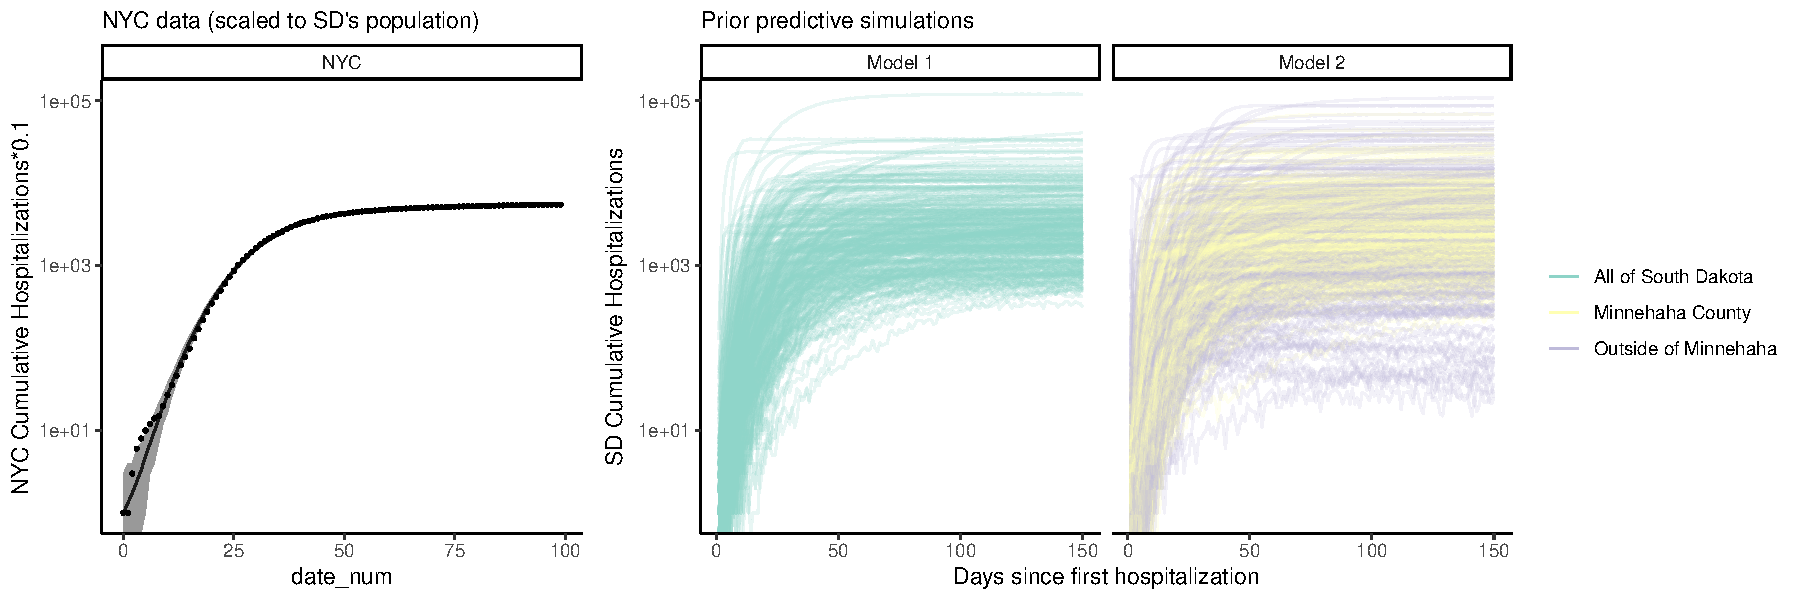
\includegraphics{test_files/figure-latex/plot-nyc-1.pdf}
\caption{\label{fig:plot-nyc}Left: Model of New York City's hospitalization curve. Data are divided by 10 to reflect the relative population sizes in South Dakota versus New York city. Three-hundred simulations of cumulative hospitalizations from the prior predictive distribution of each model. Priors for Model 1 were derived from the fit of NYC's hospitalization curve. Priors for Model 2 were similar to those of Model 1, but had a reduced prediction of cumulative hospitalizations to account for the smaller populations of each group (Minnehaha County vs Outside Minnehaha County) relative to the whole state population.\label{prior:plot}}
\end{figure}

\begin{figure}
\centering
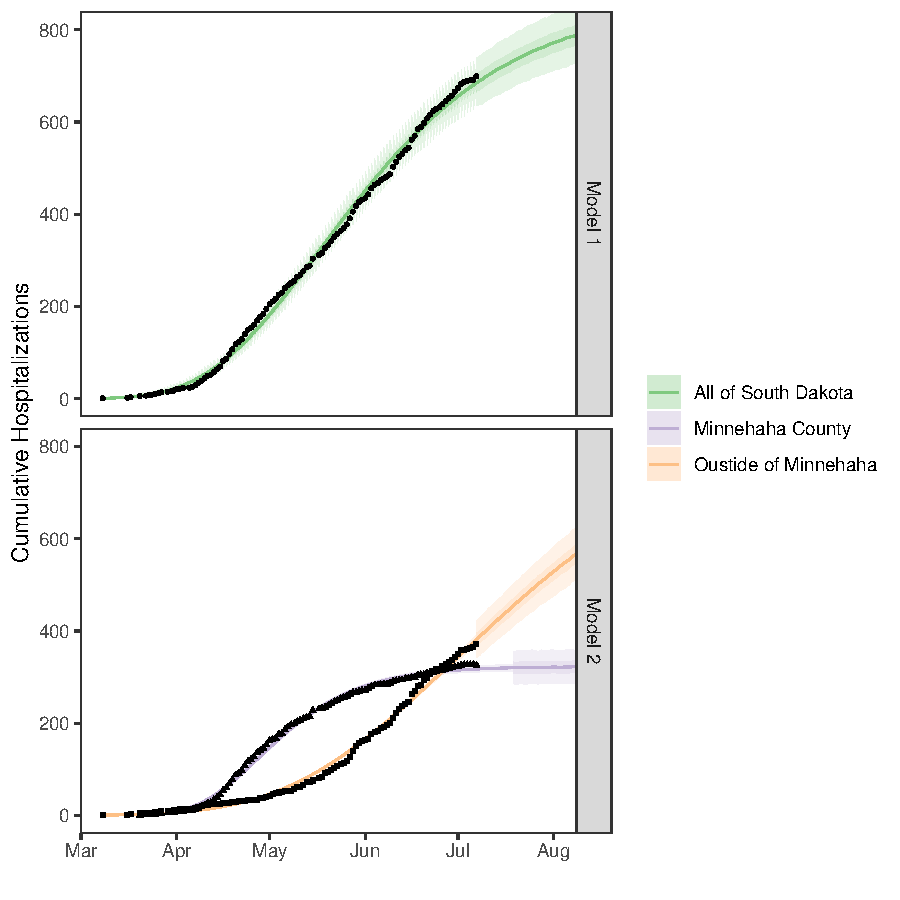
\includegraphics{test_files/figure-latex/Plot posteriors and priors-1.pdf}
\caption{(\#fig:Plot posteriors and priors)Posterior distributions of cumulative hospitalizations in South Dakota. Lines indicate medians and shading indicates the 50 and 90\% intervals. Predictions beyond the data represent samples from the posterior predictive distribution. Predictions within the data represent samples from the posterior fitted distribution.\label{post_all:plot}}
\end{figure}

\begin{figure}
\centering
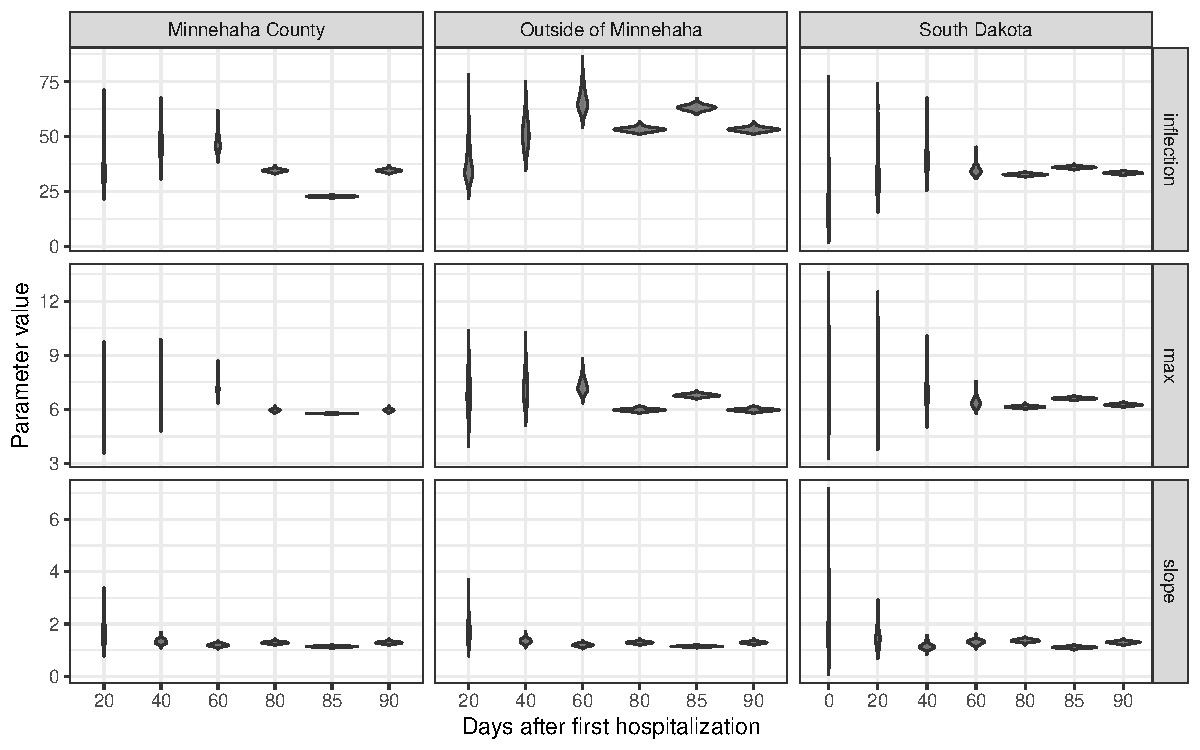
\includegraphics{test_files/figure-latex/unnamed-chunk-3-1.pdf}
\caption{\label{fig:unnamed-chunk-3}Change in parameter values over time. Violins represent posterior distributions of parameter values (untransformed) over time as models are fit using data at day 0, 20, 40, 60, 80, 100, and the most recent date.\label{param_time_plot:plot}}
\end{figure}

\begin{figure}
\centering
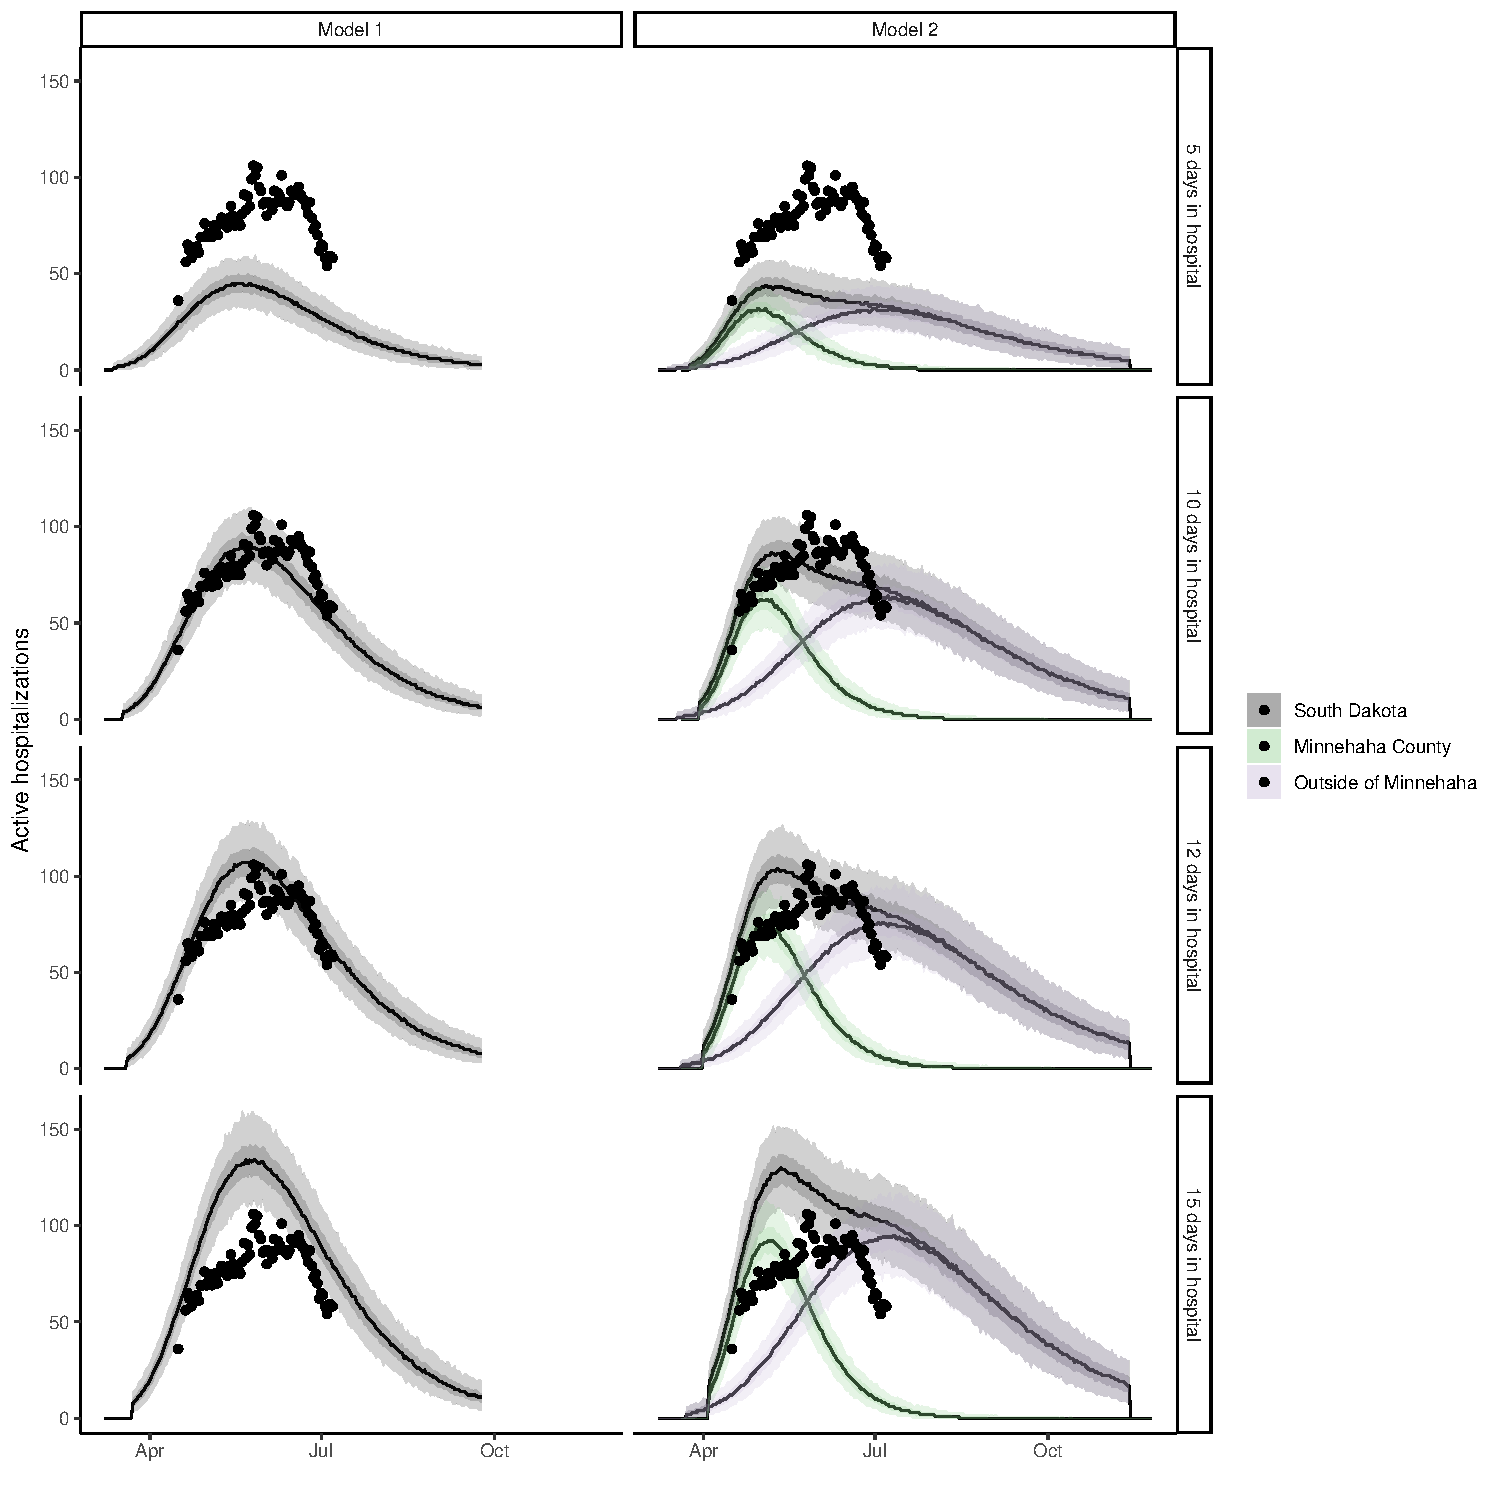
\includegraphics{test_files/figure-latex/unnamed-chunk-4-1.pdf}
\caption{\label{fig:unnamed-chunk-4}Posterior predictive distributions of active hospitalizations in South Dakota. Lines indicate medians and shading indicates the 50 and 95\% prediction intervals.\label{active_daily_group:plot}}
\end{figure}

\end{document}
